%%%%%%%%%%%%%%%%%%%%%%%%%%%%%%%%%%%%%%%%%%%%%%%%%%
% Basic setup. Most papers should leave these options alone.
\documentclass[fleqn,usenatbib]{mnras}

% MNRAS is set in Times font. If you don't have this installed (most LaTeX
% installations will be fine) or prefer the old Computer Modern fonts, comment
% out the following line
\usepackage{newtxtext,newtxmath}
% Depending on your LaTeX fonts installation, you might get better results with one of these:
%\usepackage{mathptmx}
%\usepackage{txfonts}

% Use vector fonts, so it zooms properly in on-screen viewing software
% Don't change these lines unless you know what you are doing
\usepackage[T1]{fontenc}

% Allow "Thomas van Noord" and "Simon de Laguarde" and alike to be sorted by "N" and "L" etc. in the bibliography.
% Write the name in the bibliography as "\VAN{Noord}{Van}{van} Noord, Thomas"
\DeclareRobustCommand{\VAN}[3]{#2}
\let\VANthebibliography\thebibliography
\def\thebibliography{\DeclareRobustCommand{\VAN}[3]{##3}\VANthebibliography}


%%%%% AUTHORS - PLACE YOUR OWN PACKAGES HERE %%%%%

% Only include extra packages if you really need them. Common packages are:
\usepackage{graphicx}	% Including figure files
\usepackage{amsmath}	% Advanced maths commands
\usepackage{amssymb}	% Extra maths symbols

%%%%%%%%%%%%%%%%%%%%%%%%%%%%%%%%%%%%%%%%%%%%%%%%%%

%%%%% AUTHORS - PLACE YOUR OWN COMMANDS HERE %%%%%

% Please keep new commands to a minimum, and use \newcommand not \def to avoid
% overwriting existing commands. Example:
%\newcommand{\pcm}{\,cm$^{-2}$}	% per cm-squared

%%%%%%%%%%%%%%%%%%%%%%%%%%%%%%%%%%%%%%%%%%%%%%%%%%

%%%%%%%%%%%%%%%%%%% TITLE PAGE %%%%%%%%%%%%%%%%%%%

% Title of the paper, and the short title which is used in the headers.
% Keep the title short and informative.
\title[Hot Accretion in FIRE]{Galactic discs fed by hot accretion in the FIRE simulations}

% The list of authors, and the short list which is used in the headers.
% If you need two or more lines of authors, add an extra line using \newauthor
\author[\ldots]{
\ldots,$^{1}$\thanks{E-mail: mn@ras.org.uk (KTS)}
\\
% List of institutions
$^1$ \ldots
}

% These dates will be filled out by the publisher
\date{Accepted XXX. Received YYY; in original form ZZZ}

% Enter the current year, for the copyright statements etc.
\pubyear{2020}

% Don't change these lines

\newcommand{\Rcon}{R_{T=10^5\,{\rm K}}}
\newcommand{\tcon}{t_{T=10^5\,{\rm K}}}
\newcommand{\Mdot}{\dot{M}}
\newcommand{\Rcirc}{R_{\rm circ}} %need better name as R_cool means something else
\newcommand{\Rvir}{R_{\rm vir}}
\newcommand{\nH}{n_{\rm H}}

\begin{document}
\label{firstpage}
\pagerange{\pageref{firstpage}--\pageref{lastpage}}
\maketitle

% Abstract of the paper
\begin{abstract}
We study how gas accretes onto $\sim L^\star$ star-forming galaxies at redshift $z\sim0$ using the FIRE cosmological simulations.
We evaluate the relative importance of three different modes of accretion: 
gas that never heats to the virial temperature (``cold accretion''), 
cool clouds which condense out of the hot halo, lose buoyancy and accrete  (``condensation''), 
and inflowing hot gas which remains hot down to the galaxy scale (``cooling flow'').
We demonstrate that across our sample of MW-mass halos most accretion occurs via a cooling flow.
% We demonstrate that across our sample of $xx$ MW-mass halos most accretion occurs via a cooling flow, accounting for $yy-zz\%$ of all accreted gas. % Put this back in when we know the numbers
Gas accreted in this mode is hot and quasi-spherical down to when it becomes rotationally-supported at $\lesssim 0.1$ of the halo virial radius.
After becoming rotationally-supported it simultaneously cools and circularizes, thus joining the outskirts of the galactic disc. 
% Only a small fraction ($zz$\%) of this hot flow experienced condensation and reheating prior to accretion. 
% The remaining $vv-ww\%$ of accreted gas originates in cool clouds which condensed out of the halo. Cold accretion does not occur in appreciable quantities at $z\sim0$ in our simulations.
\textbf{
Include: Compare Mdotcool with the accretion rate and SFR to further strengthen the relation, maybe through Figure 1 in an energetic sense.
}
\end{abstract}

% Select between one and six entries from the list of approved keywords.
% Don't make up new ones.
\begin{keywords}
keyword1 -- keyword2 -- keyword3
\end{keywords}

%%%%%%%%%%%%%%%%%%%%%%%%%%%%%%%%%%%%%%%%%%%%%%%%%%

%%%%%%%%%%%%%%%%% BODY OF PAPER %%%%%%%%%%%%%%%%%%

\subsection{ KEY FOR COAUTHORS}
\textbf{Bold: Notes for things to implement.} \\
\textit{Italics: Rough text, needs polishing.} \\
Normal: Normal text, polished enough to be included in a draft.

\section{Introduction}

% Accretion in cosmological simulations
\textbf{Ho,Martin+2019}

% Angular momentum in cosmo sims
\textbf{DeFelippis' work}

% C-A comments
\textbf{
Galaxies have lower j than the CGM due to preferential accretion of low-j gas.
Low angular momentum gas is more likely to form stars because it moves inwards and increases density.
https://ui.adsabs.harvard.edu/abs/2019MNRAS.488.4801J/abstract
https://ui.adsabs.harvard.edu/abs/2015MNRAS.449.2087D/abstract
this paper also discusses/assumes low sAM gas preferentially ends up in stars:
https://ui.adsabs.harvard.edu/abs/2017MNRAS.466.1625Z/abstract
}

% Modes of hot accretion
\textit{
Two modes of hot accretion:
\begin{itemize}
    \item condensation (Maller \& Bullock 2004; Kaufmann, Bullock+09; McCourt+12; Voit+17)
    \item classic CF (Cowie+80; Paper I)
\end{itemize}
}
\textbf{Intro TBD}

\textbf{Info-dump from Jonathan:}
Some refs on truncation radius in observations:
\cite{Kregel2002} tight correlation between disk truncation radius and Re (Spearman 0.95) in 34 edge-on spirals (in face-on galaxies stellar halos can outshine truncation, see Martín-Navarro+14). $R_{\rm truncation} / R_e({\rm Iband}) \sim~ 3.6$. Somewhat higher ratio in small Re spirals, somewhat lower ratio in bluer passbands (where Re is larger).
Re is independently found to be proportional to the virial radius, roughly Re ~ 0.015 Rvir (e.g. Kravtsov13).
Martín-Navarro+12: 34 edge-on spirals from SDSS / S4G: Rtruncation ~ 1.1 R25, where R25 is the radius at which the surface brightness equals 25mag
van der Kruit+07: when a HI-warp is present in the gaseous disc it starts at 1.1 Rtrunc; the truncation radius and the onset of the warps coincide radially sometimes with features in the rotation curve and often with steep declines in the HI surface density; inner disks are very flat and the onset of the warp just beyond the truncation radius is abrupt and discontinuous;
Perez+04, Trujillo\&Pohlen05, Azzollini+08: measurements of truncation radius at z~1
Comeron+12: 70 edge-on S4G galaxies. 77\% of thin discs truncate, but only 31\% of thick discs. $M_thick/M_thin$ increases with decreasing $v_c$
de Jong+07: Stellar Populations across the NGC 4244 Truncated Galactic Disk
Haberzettl+07: truncation in LSBs
some suggested theoretical explanations of breaks:
https://ui.adsabs.harvard.edu/abs/2009MNRAS.398..591S/abstract
https://ui.adsabs.harvard.edu/abs/2008ApJ...675L..65R/abstract
https://ui.adsabs.harvard.edu/abs/2006ApJ...645..209D/abstract
https://ui.adsabs.harvard.edu/abs/2009ApJ...705L.133M/abstract
https://ui.adsabs.harvard.edu/abs/1987A%26A...173...59V/abstract
and short summary sentence from Comeron+12 intro:
"Several theories compete for explaining the origin of such breaks. Truncations have been explained by dynamical arguments related to the conservation of angular momentum during galaxy formation, by star formation thresholds, and by the redistribution of angular momentum by a bar. Antitruncations have in some cases been linked to interactions and mergers."
Antitruncations are cases where the Surface Brightness profiles flattens at large disc radii rather than steepens. From my impression of the observational literature anti-truncations are seen mainly in face-on galaxies and are related to the existence of stellar halos

\section{Methods}

% Simulation sample
\textit{
We use four simulations:
m12i\_md\_7100, m12b\_md\_7100, m12f\_core\_7100, m12m\_core\_7100
}
\textbf{Also do massive galaxies?}
\textbf{Do more metal diffusion simulations (the non-md sims have unexpected cooling at large radii): at least 4 metal diffusion simulations would be good.}

% How we select the particles
\textit{
For a given galaxy we select all particles that are in the central galaxy at $z=0$ and in the CGM 1 Gyr prior.
The galaxy is defined as all gas and stars inside $R_{\rm gal} = 0.1 R_{\rm vir}$, with an additional density cut of $n_{\rm H} = 0.13$ cm$^{-3}$ for gas.
The CGM is defined as all gas inside $0.1 -1 R_{\rm vir}$.
For each selected particle we retrieve the full history of the particle (including temperature, density, metallicity) throughout the simulation.
}

% Handling duplicate IDS
\textit{
Of the particles targeted to be tracked $<2\%$ are particles that will accumulate or have accumulated at least twice their mass' worth in deposited mass from stellar feedback, resulting in them being split into two particles.
These particles pose a problem for tracking because the history of the additional mass is not recorded and likely comes from a variety of sources.
As in \cite{Hafen2019}, we discard these particles, which are not expected to affect our results due to their small contribution.
}

% Definition of t1e5 and calculating it
\textit{
$\tcon$ is the latest time among our particles at which the particle transitions from $T > 10^5$ K to $T< 10^5$ K.
When selecting values in the simulation corresponding to $\tcon$ we use the last snapshot an accreted particle had $T > 10^5$ K, i.e. the snapshot immediately before the transition.
Note that we do not account for gas particles being heated to $T > 10^5$ K while still in the ISM.
Because our sample of tracked particles focuses on recently accreted particles this is expected to be a small population that will not contaminate our analysis.
This is confirmed after-the-fact in Figure~\ref{f: theta vs R}, where gas is not preferentially oriented in a disky ISM prior to $\tcon$.
}

% Rcon and interpretation
\textit{
Another important quantity is $\Rcon\equiv R(\tcon)$, the 3D distance from the center of the galaxy of the particle at time $\tcon$.
For gas that cools in the halo $\Rcon$  will be at CGM scales, while for gas that cools directly onto the galaxy $\Rcon$ will be at galaxy scales.
}

\section{Results}

\subsection{Phase of inflowing gas}

We calculate the mass inflow rate as
\begin{equation}\label{e:Mdot}
     \Mdot = \frac{\int_{\rm shell} v_r dm}{\Delta r} = \frac{M_{\rm shell}}{\Delta r} \langle v_r\rangle_\rho
\end{equation}
where $\Delta r$ is the shell thickness, and the integration is done on all particles which center is within the shell. Mass-weighted averaging is noted by $\langle\cdot\rangle_\rho$.

\subsection{Morphology of accreting gas}

\subsubsection{Gas cools at or near the galaxy edge}

\subsubsection{Gas forms a disk as it cools}

\subsection{Cooling and accretion mechanisms}

\textbf{TBD: $\dot{M}_{\rm stars}$ in Fig.~\ref{f:Mdot} is currently SFR$/2$. Change to SFR minus gas returned from winds/SNe.}
    
\begin{figure*}
    \centering
    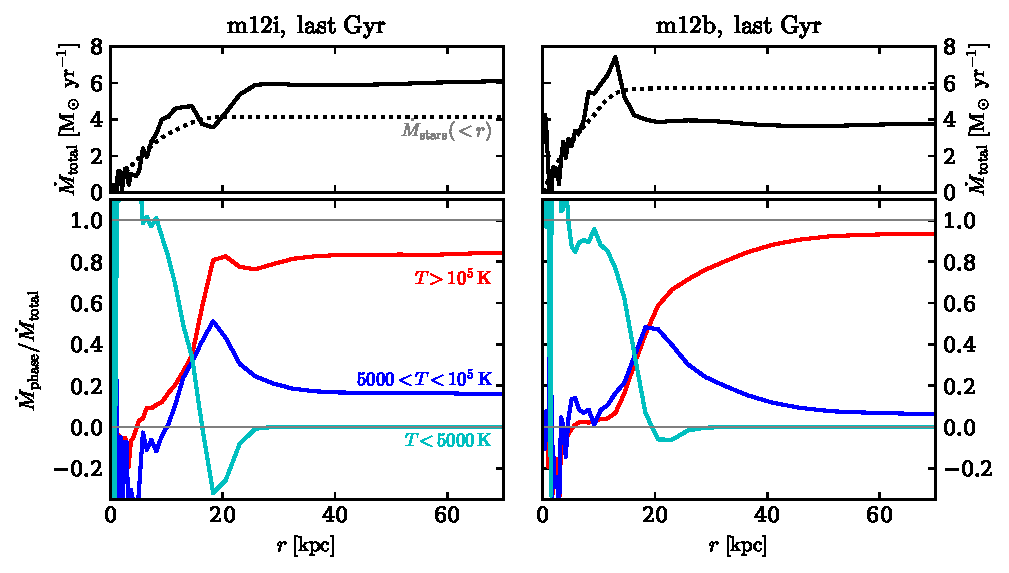
\includegraphics{Mdot_normalized.pdf}
    \caption{
    Average mass inflow rate in the last Gyr of two FIRE simulations.
    Black lines in the top panels show the total $\dot{M}_{\rm inflows}$  while colored lines in the bottom panels show the division into the hot, cool and cold phases. 
    The inflow is dominated by hot gas at $r\gtrsim 20 $ kpc.
    For comparison the dotted line shows the rate of gas being converted into stars.
    \textbf{verify conversion SFR to Mdot\_stars, add SFR of satellites}
    % \textbf{Add images of face-on $z=0$ slice with temperature and velocity arrows.}
    % \textbf{Add top x-axis with radius in units of $\Rvir$}.
    % \textbf{Add cuts on density/temperature to avoid ISM gas causing a wide dispersion at low-r.}
    % \textbf{Change to linear space to emphasize halo. Cut out accretion shock.}
    % \textbf{Try using Clarke's entropy cut.}
    }
    \label{f:Mdot}
\end{figure*}

\begin{figure*}
    \centering
    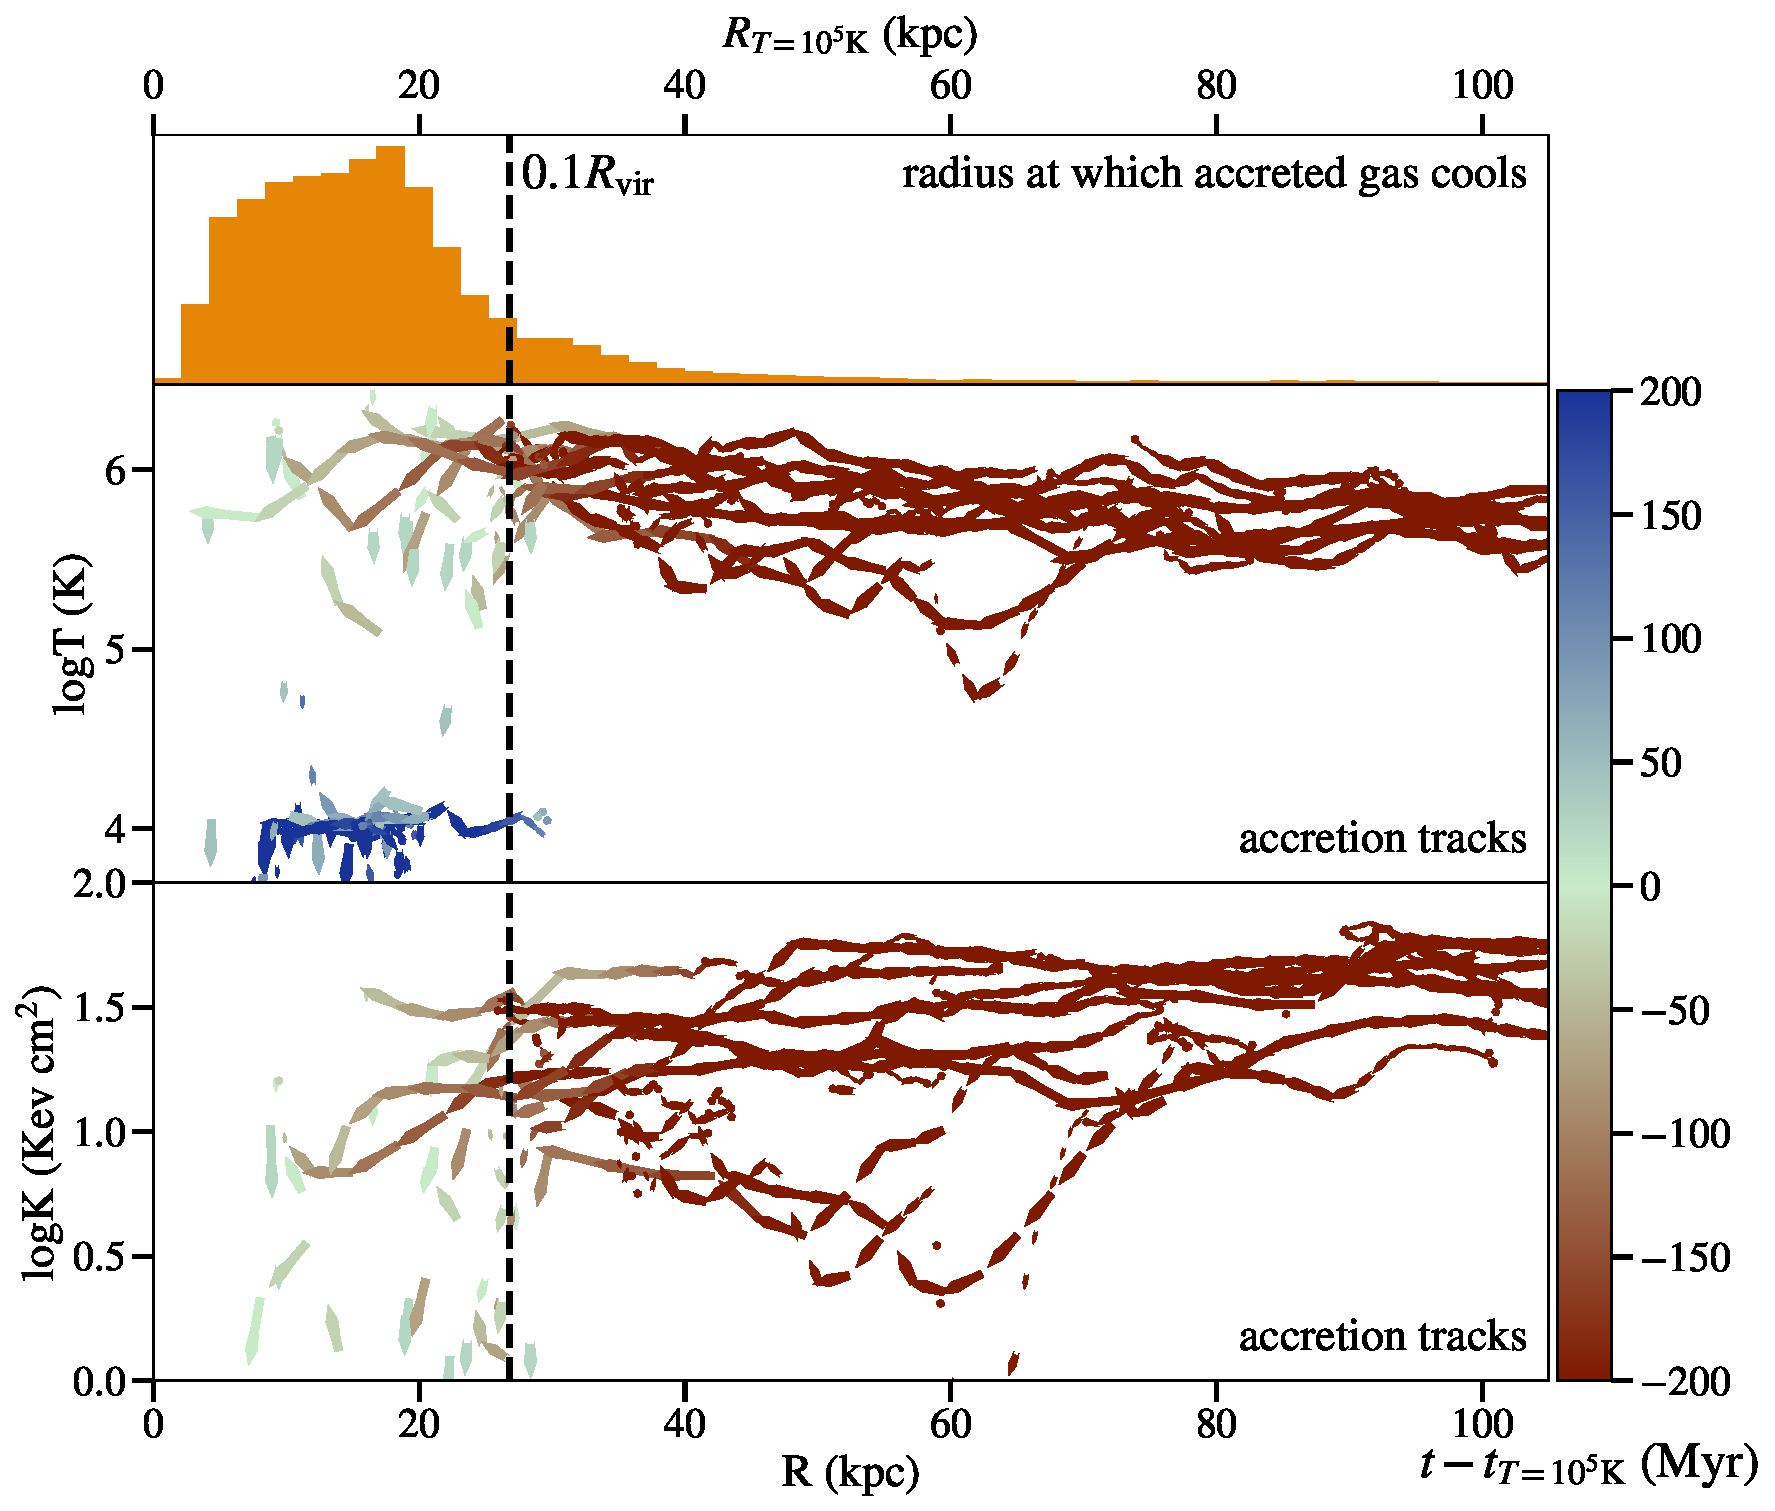
\includegraphics[width=\columnwidth]{figures/tracks_m12i_md.pdf}
    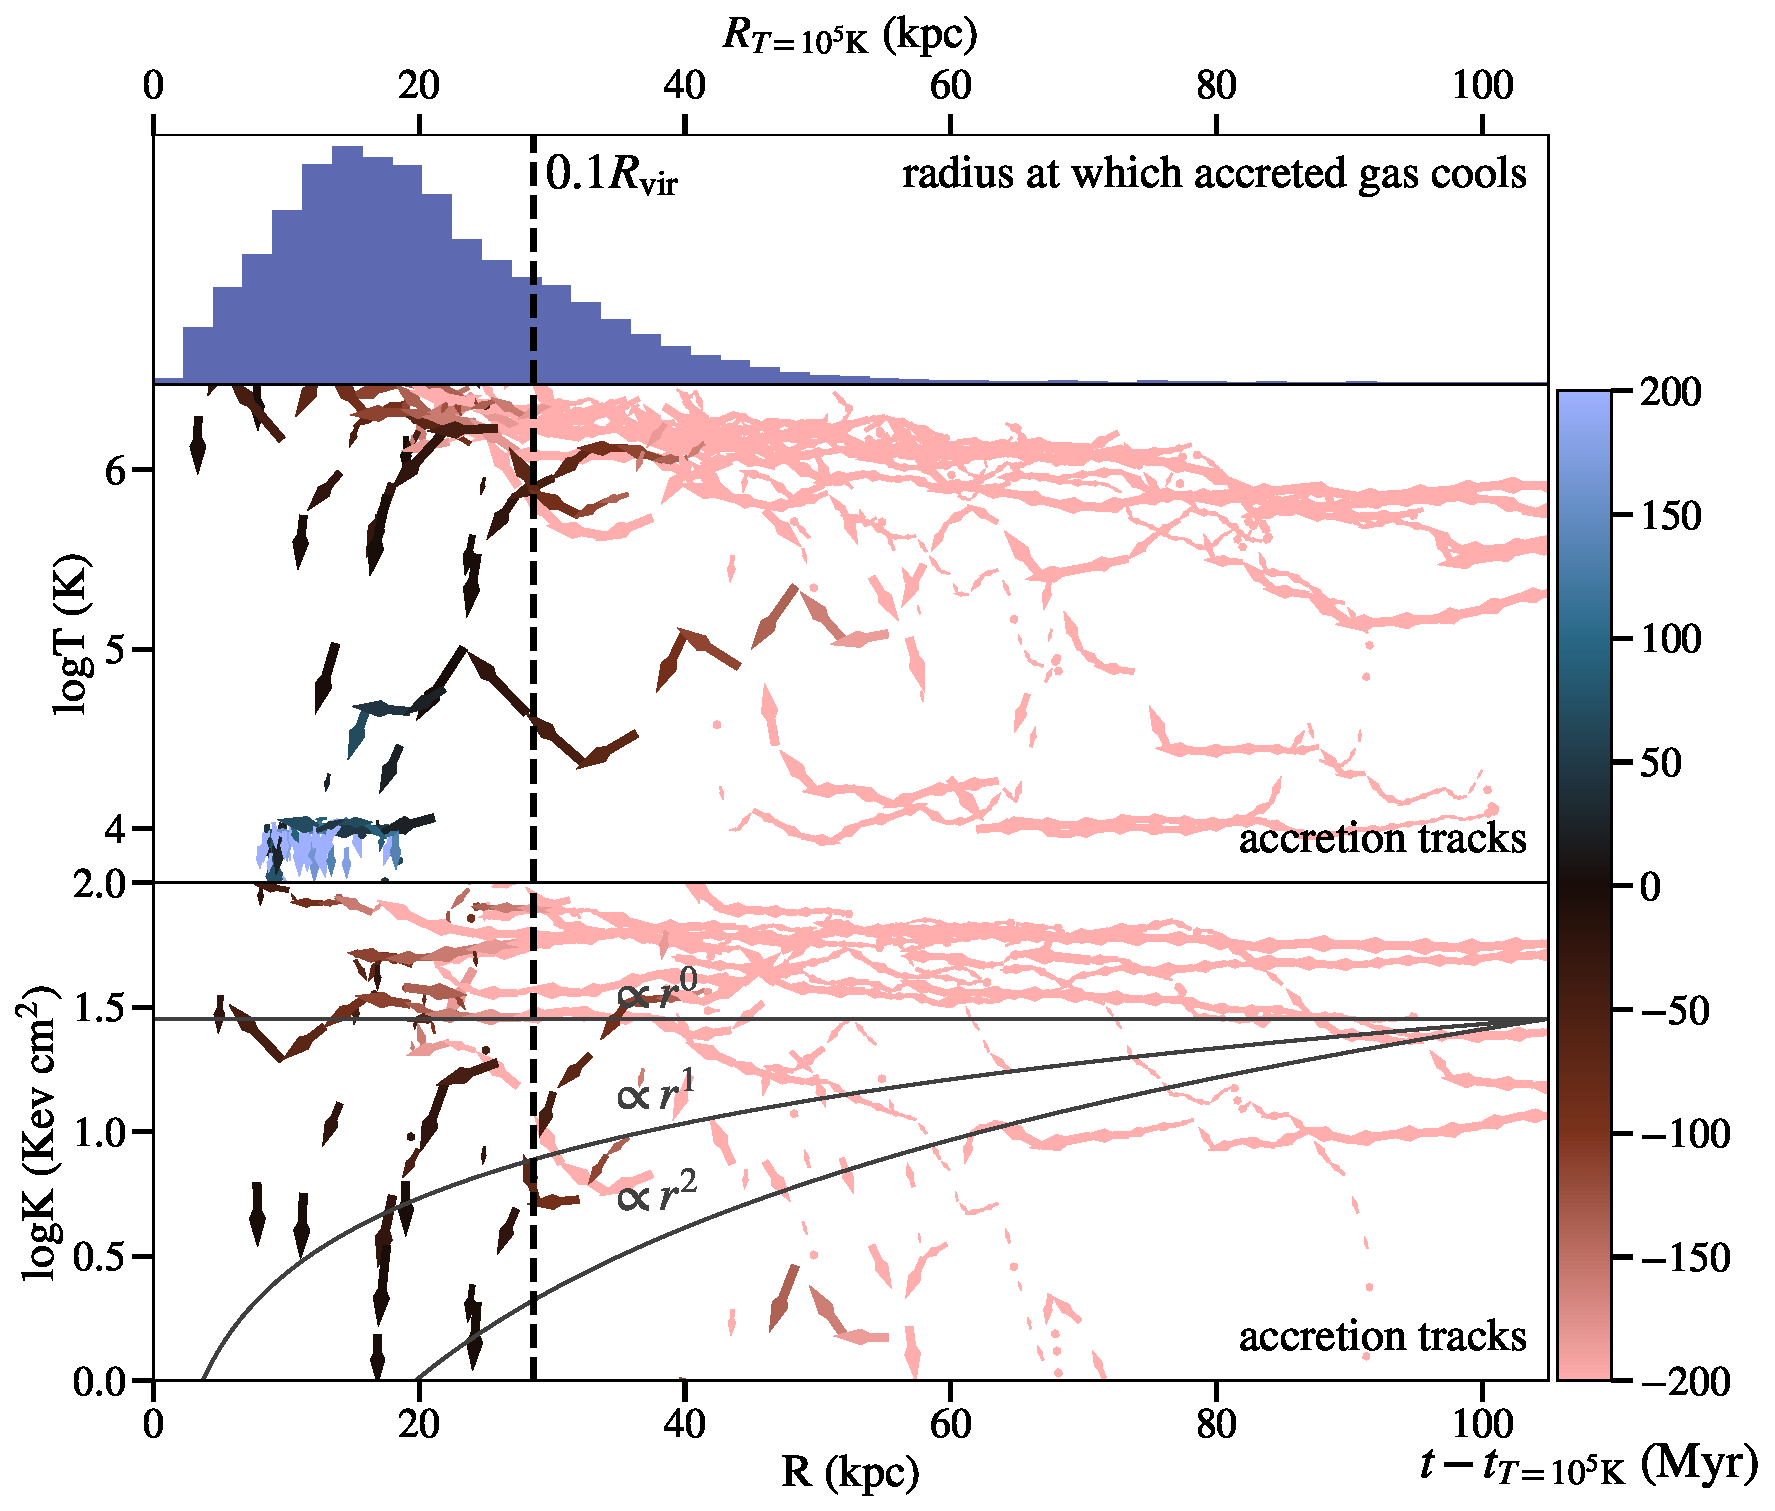
\includegraphics[width=\columnwidth]{figures/tracks_m12b_md.pdf}
    \caption{
    \textbf{Main panels:} 10 T vs.\ R and K vs.\ R tracks for two $L^\star$ halo at $z=0$, with color indicating time relative to the time at which gas cools.
    Gas either remains hot or cools only temporarily down to $\lesssim 0.1 R_{\rm vir}$. 
    % We do not show gas that has ever been ejected from the central galaxy.
    \textbf{Top panel:} Distribution of $\Rcon$, the radius at which gas particles last transitioned from $T > 10^5$ K to $T < 10^5$ K prior to accreting, i.e. the radius at which they cooled prior to accretion.
    \textbf{Try out fractional form: ultimate goal make it super clear (which the result is, so the presentation shouldn't hinder it).}
    \textbf{Remove vertical lines for Rsonic.}
    \textbf{Consider putting histograms by themselves to have a very simple, clear result with no distraction.}
    \textbf{
    Try plotting an edge-on image of the system to-scale above the histogram.
    }
    \textbf{
    Try making a 2D histogram of $\Rcon$ and the angle at which it accretes.
    }
 \textbf{Compare accretion radii (this plot) to a textbook angular momentum support radii distribution.}
    }
    \label{f: T vs R}
\end{figure*}

% \begin{figure}
%     \centering
%     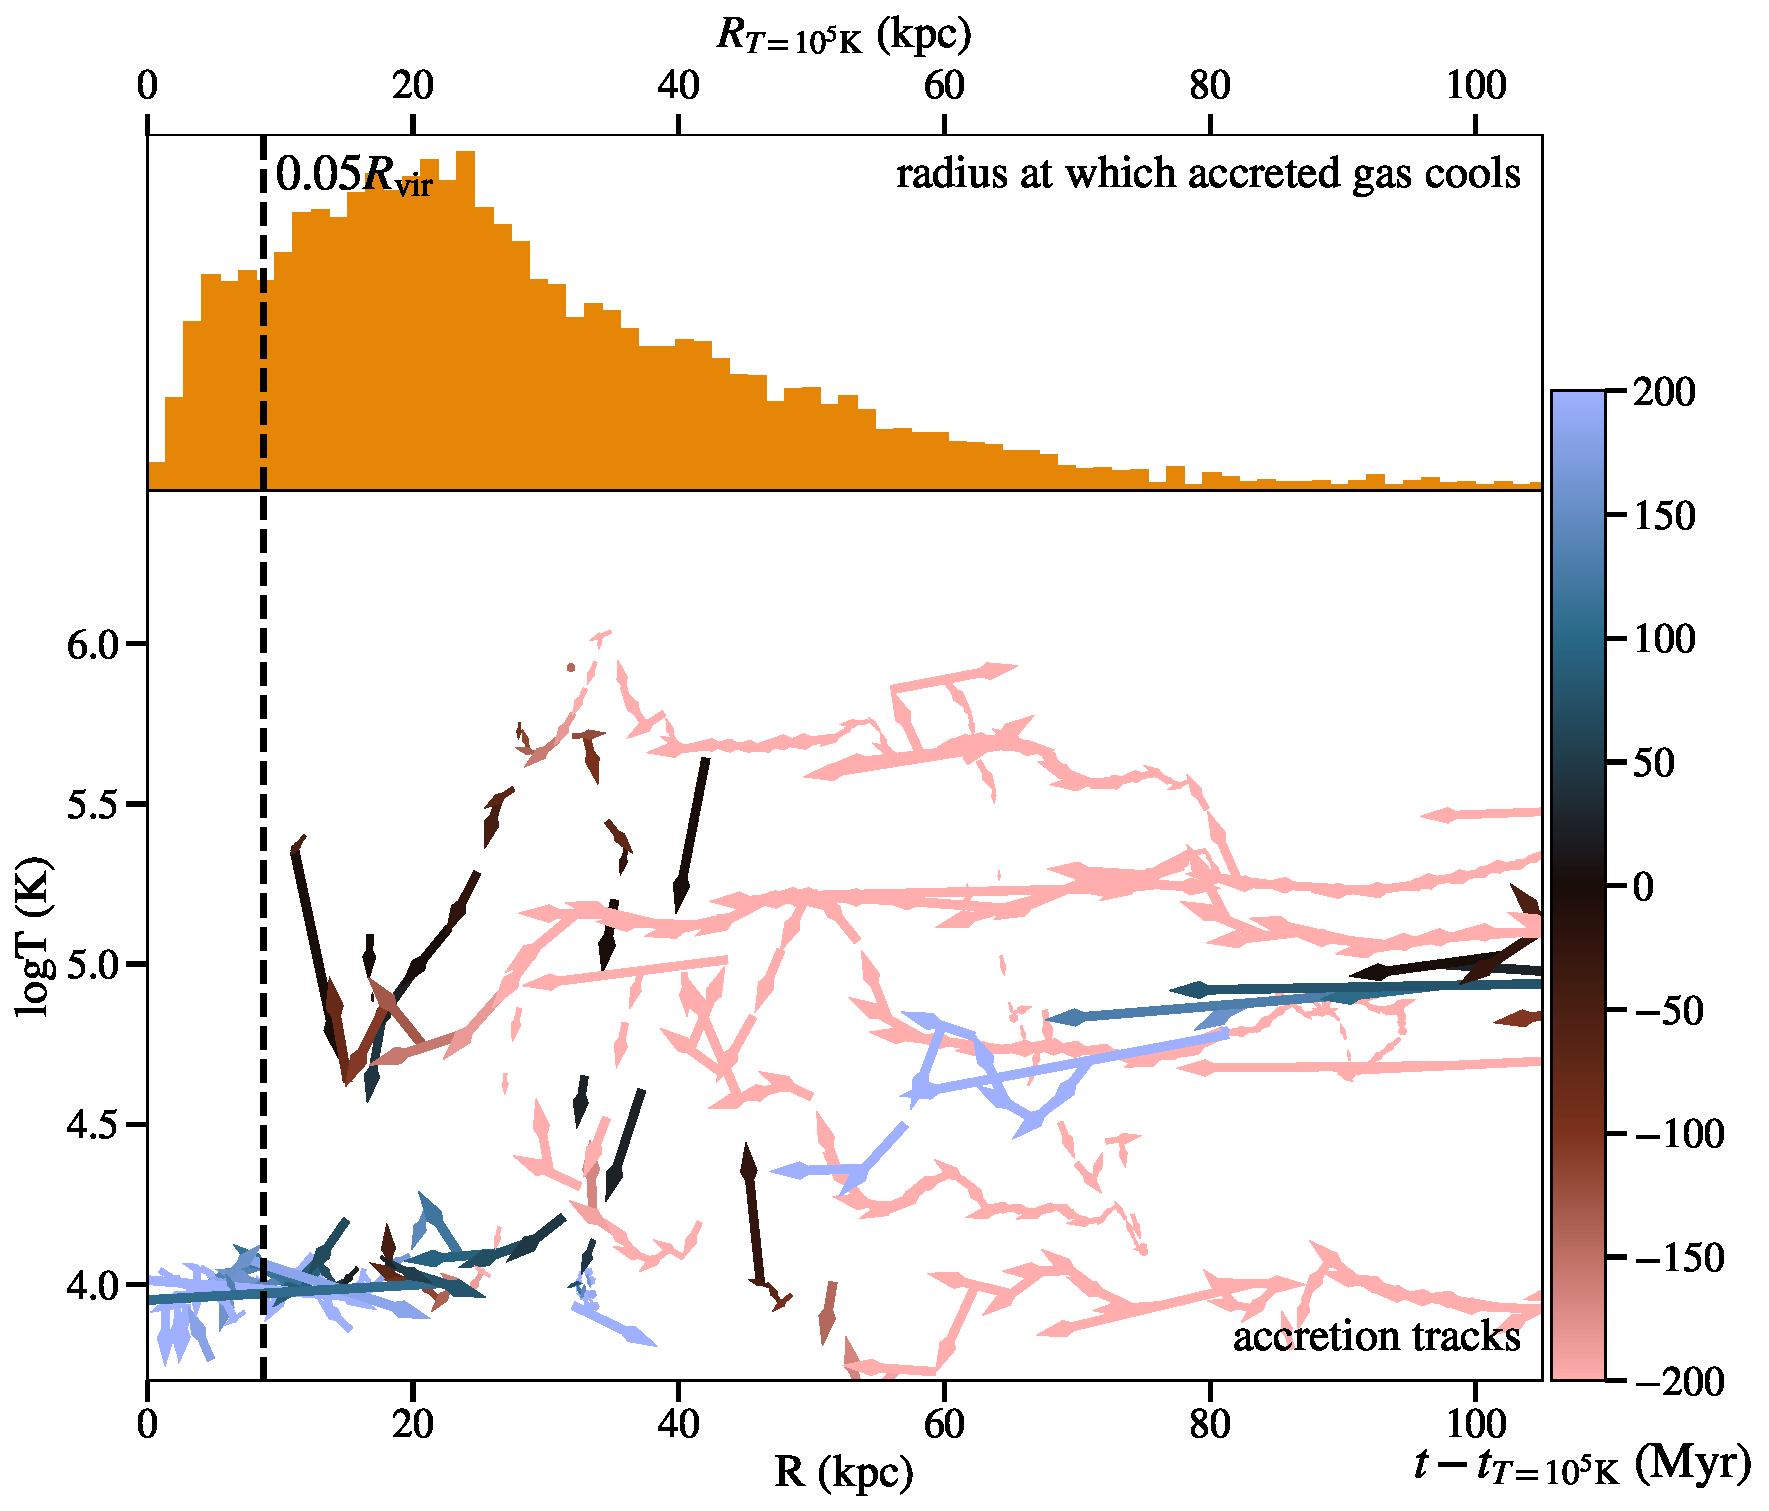
\includegraphics[width=\columnwidth]{figures/tracks_m11d_md.pdf}
%     \caption{
%     Same as Figure~\ref{f: T vs R}, but for \texttt{m11d\_md}.
%     }
%     \label{f: T vs R m11d_md}
% \end{figure}

% \begin{figure}
% \centering
% 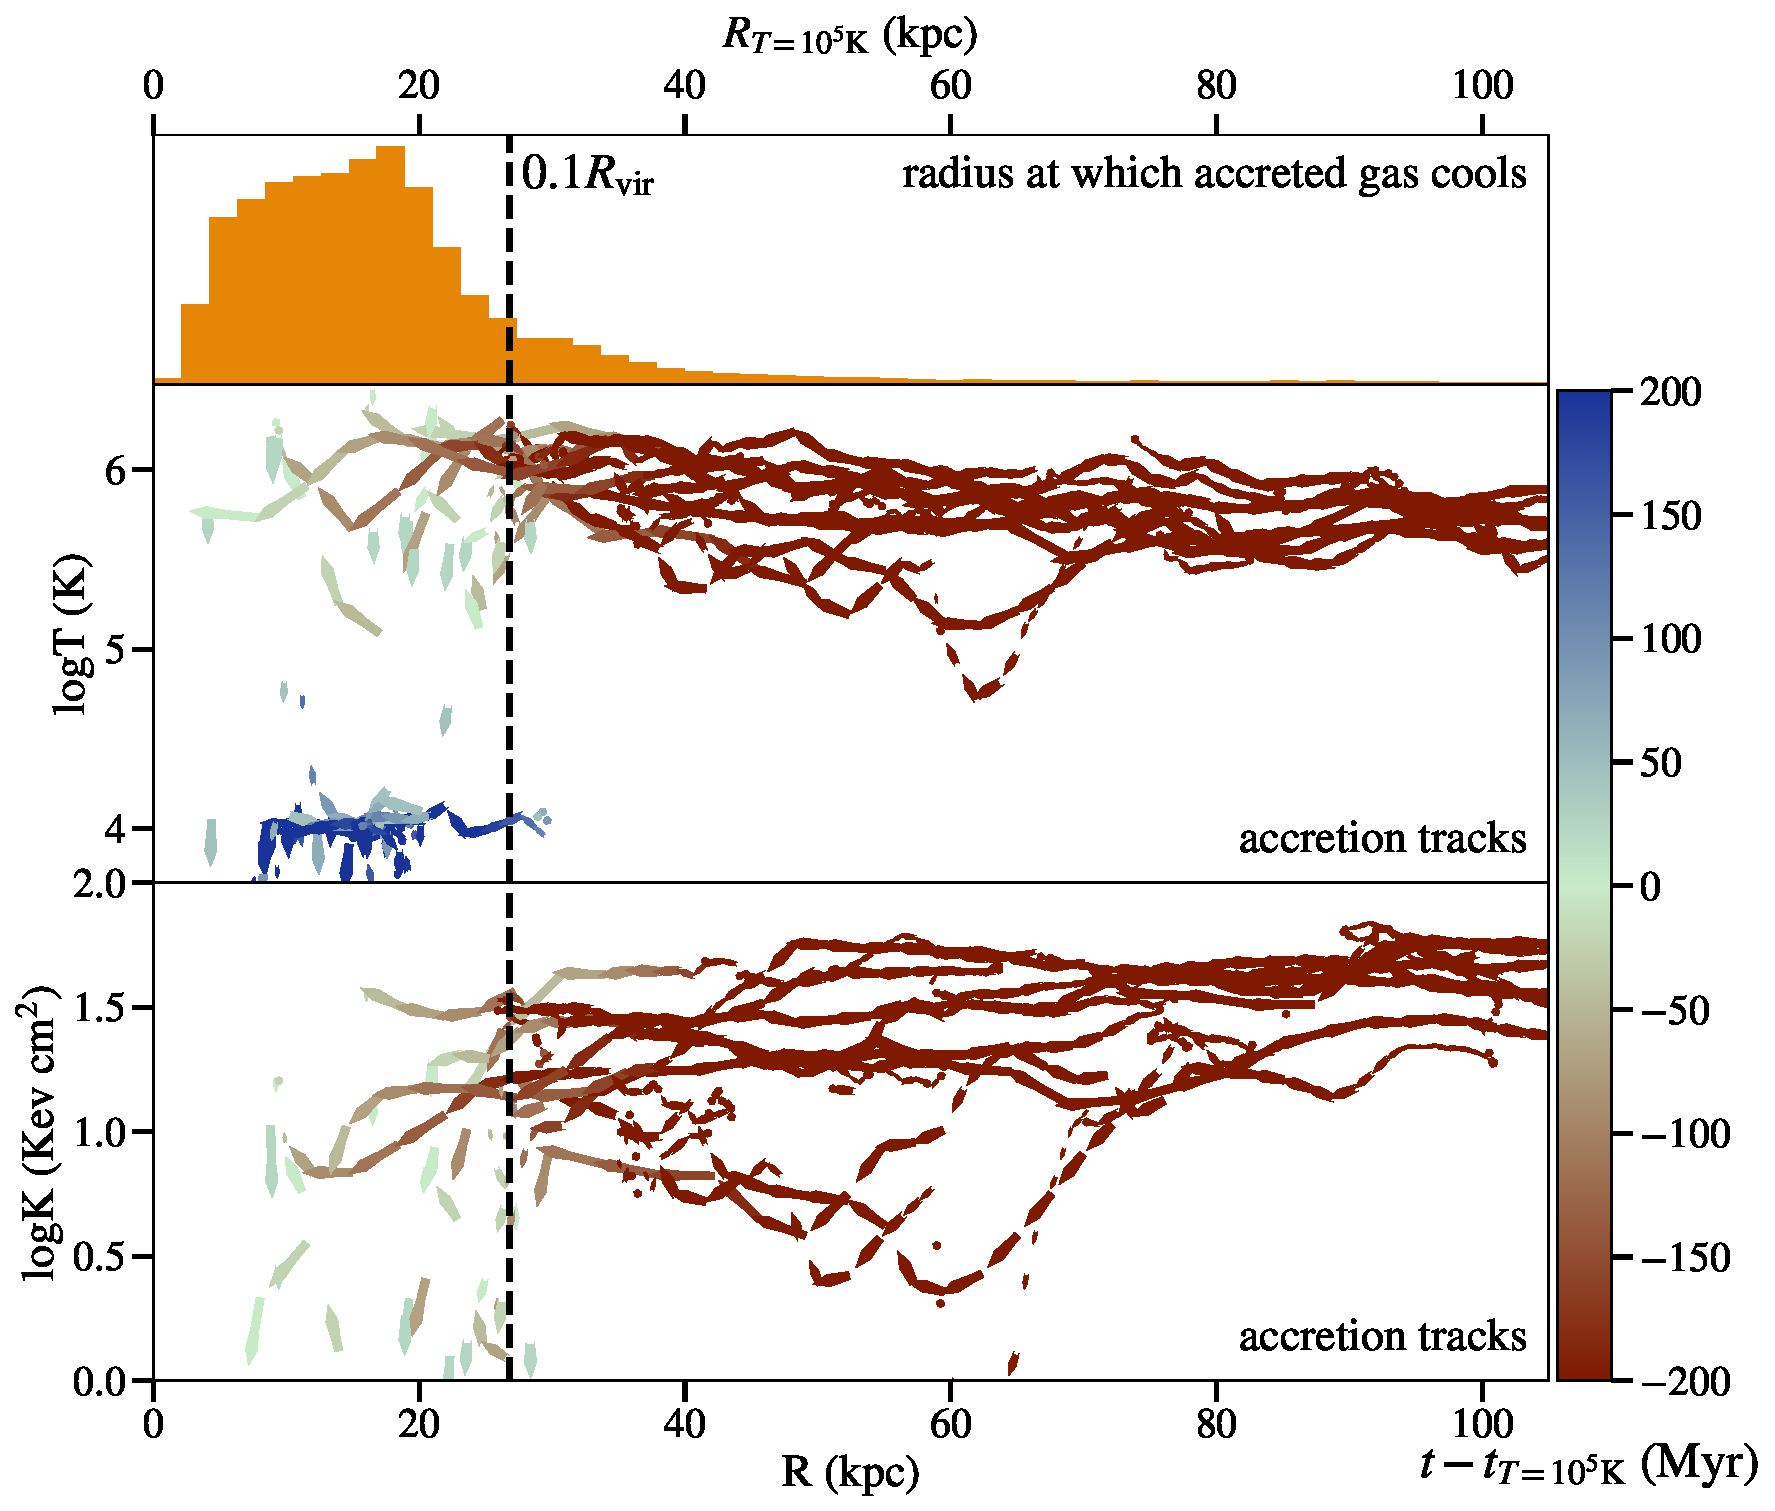
\includegraphics[width=\columnwidth]{figures/tracks_m12i_md.pdf}
% \end{figure}

\textbf{Zoom-in on axis labels for Figure 4, add ratio of radiative cooling/compressive heating.}

\begin{figure}
    \centering
    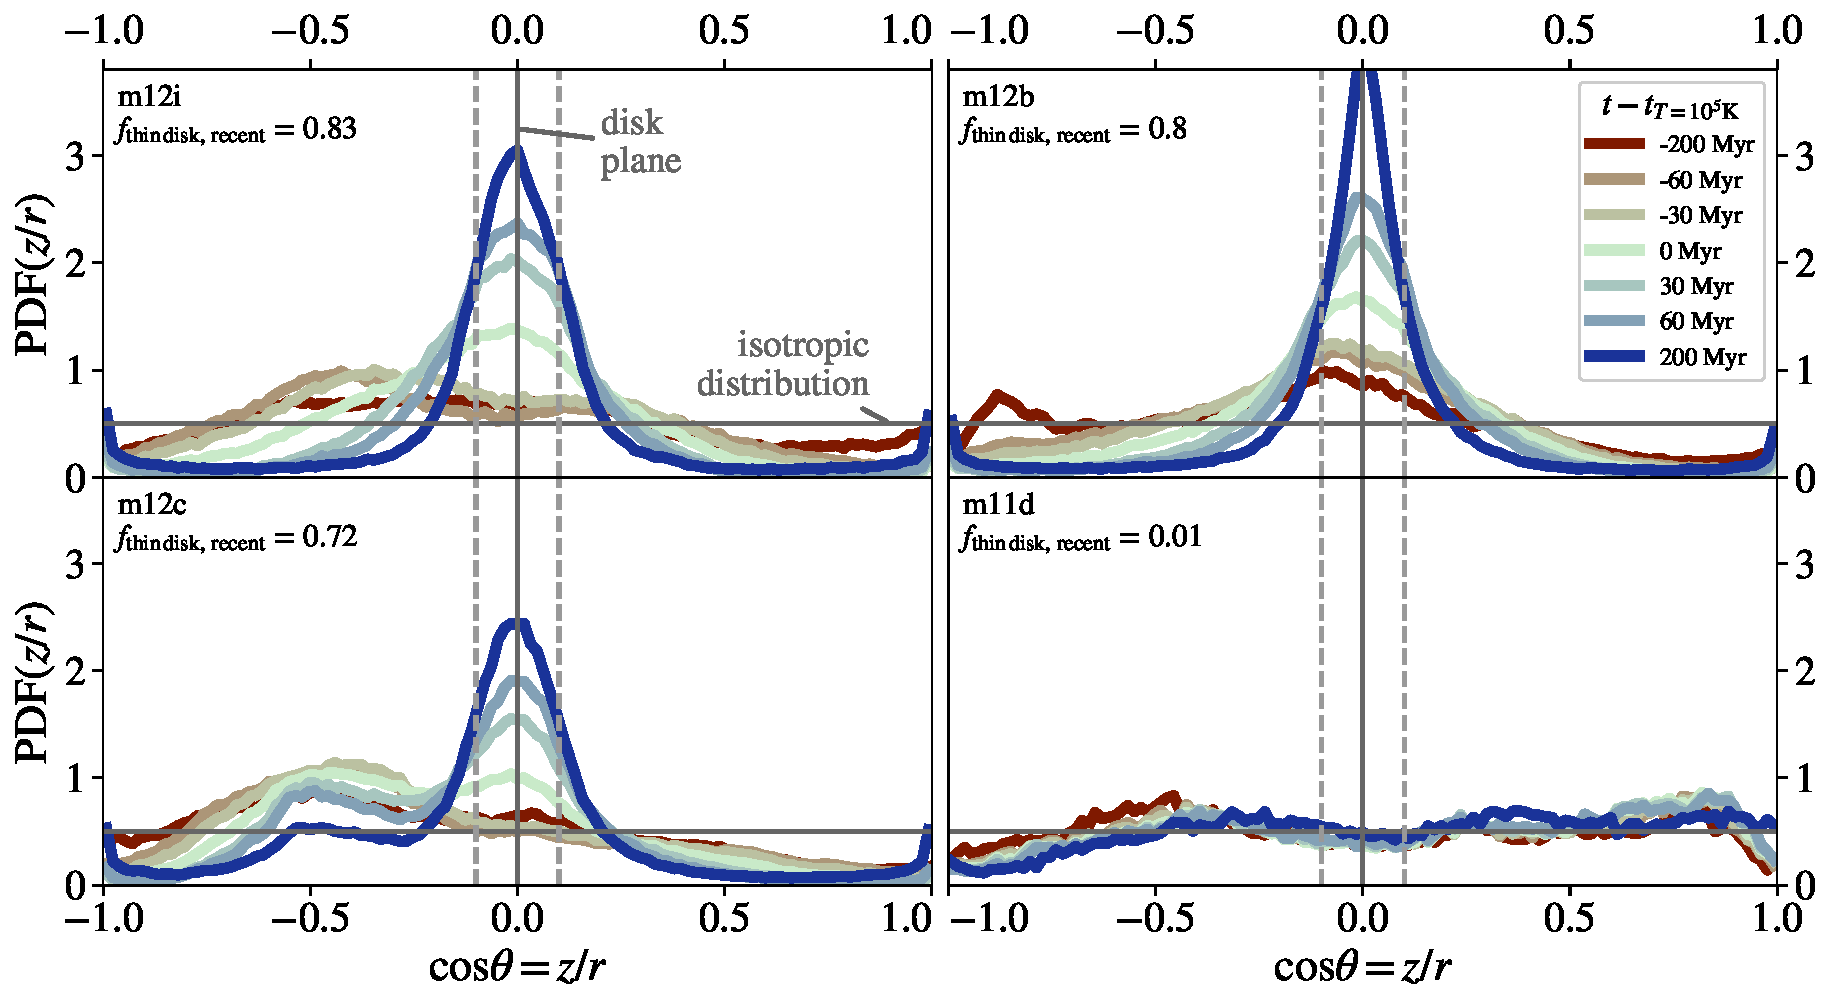
\includegraphics[width=\columnwidth]{figures/theta_vs_t.pdf}
    \caption{
    Angular distribution of accreting gas over 250 Myr before/after cooling. Cooling and circularization occur together -- prior to cooling the gas is distributed quasi-spherically, while after cooling the gas has a disc like configuration.
    \textbf{note `disc distribution' near vertical line'}.
    \textbf{Definitely m11d back in for comparison. An advantage for including is that it provides a powerful contrast.}.
    \textbf{Try splitting up into two panels side-by-side with a "before" panel and an "after" panel.}
    \textbf{Make a plot using the same particle bins as here, but showing the sum of the angular momentum for all particles in the bin, divided by vcR}
    \textbf{See if the distribution becomes narrower if selecting a narrower range of particles.}
    }
    \label{f: theta vs R}
\end{figure}

\begin{figure*}
% 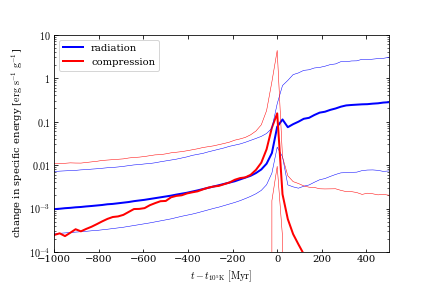
\includegraphics[width=\columnwidth]{rad_vs_compress.png}
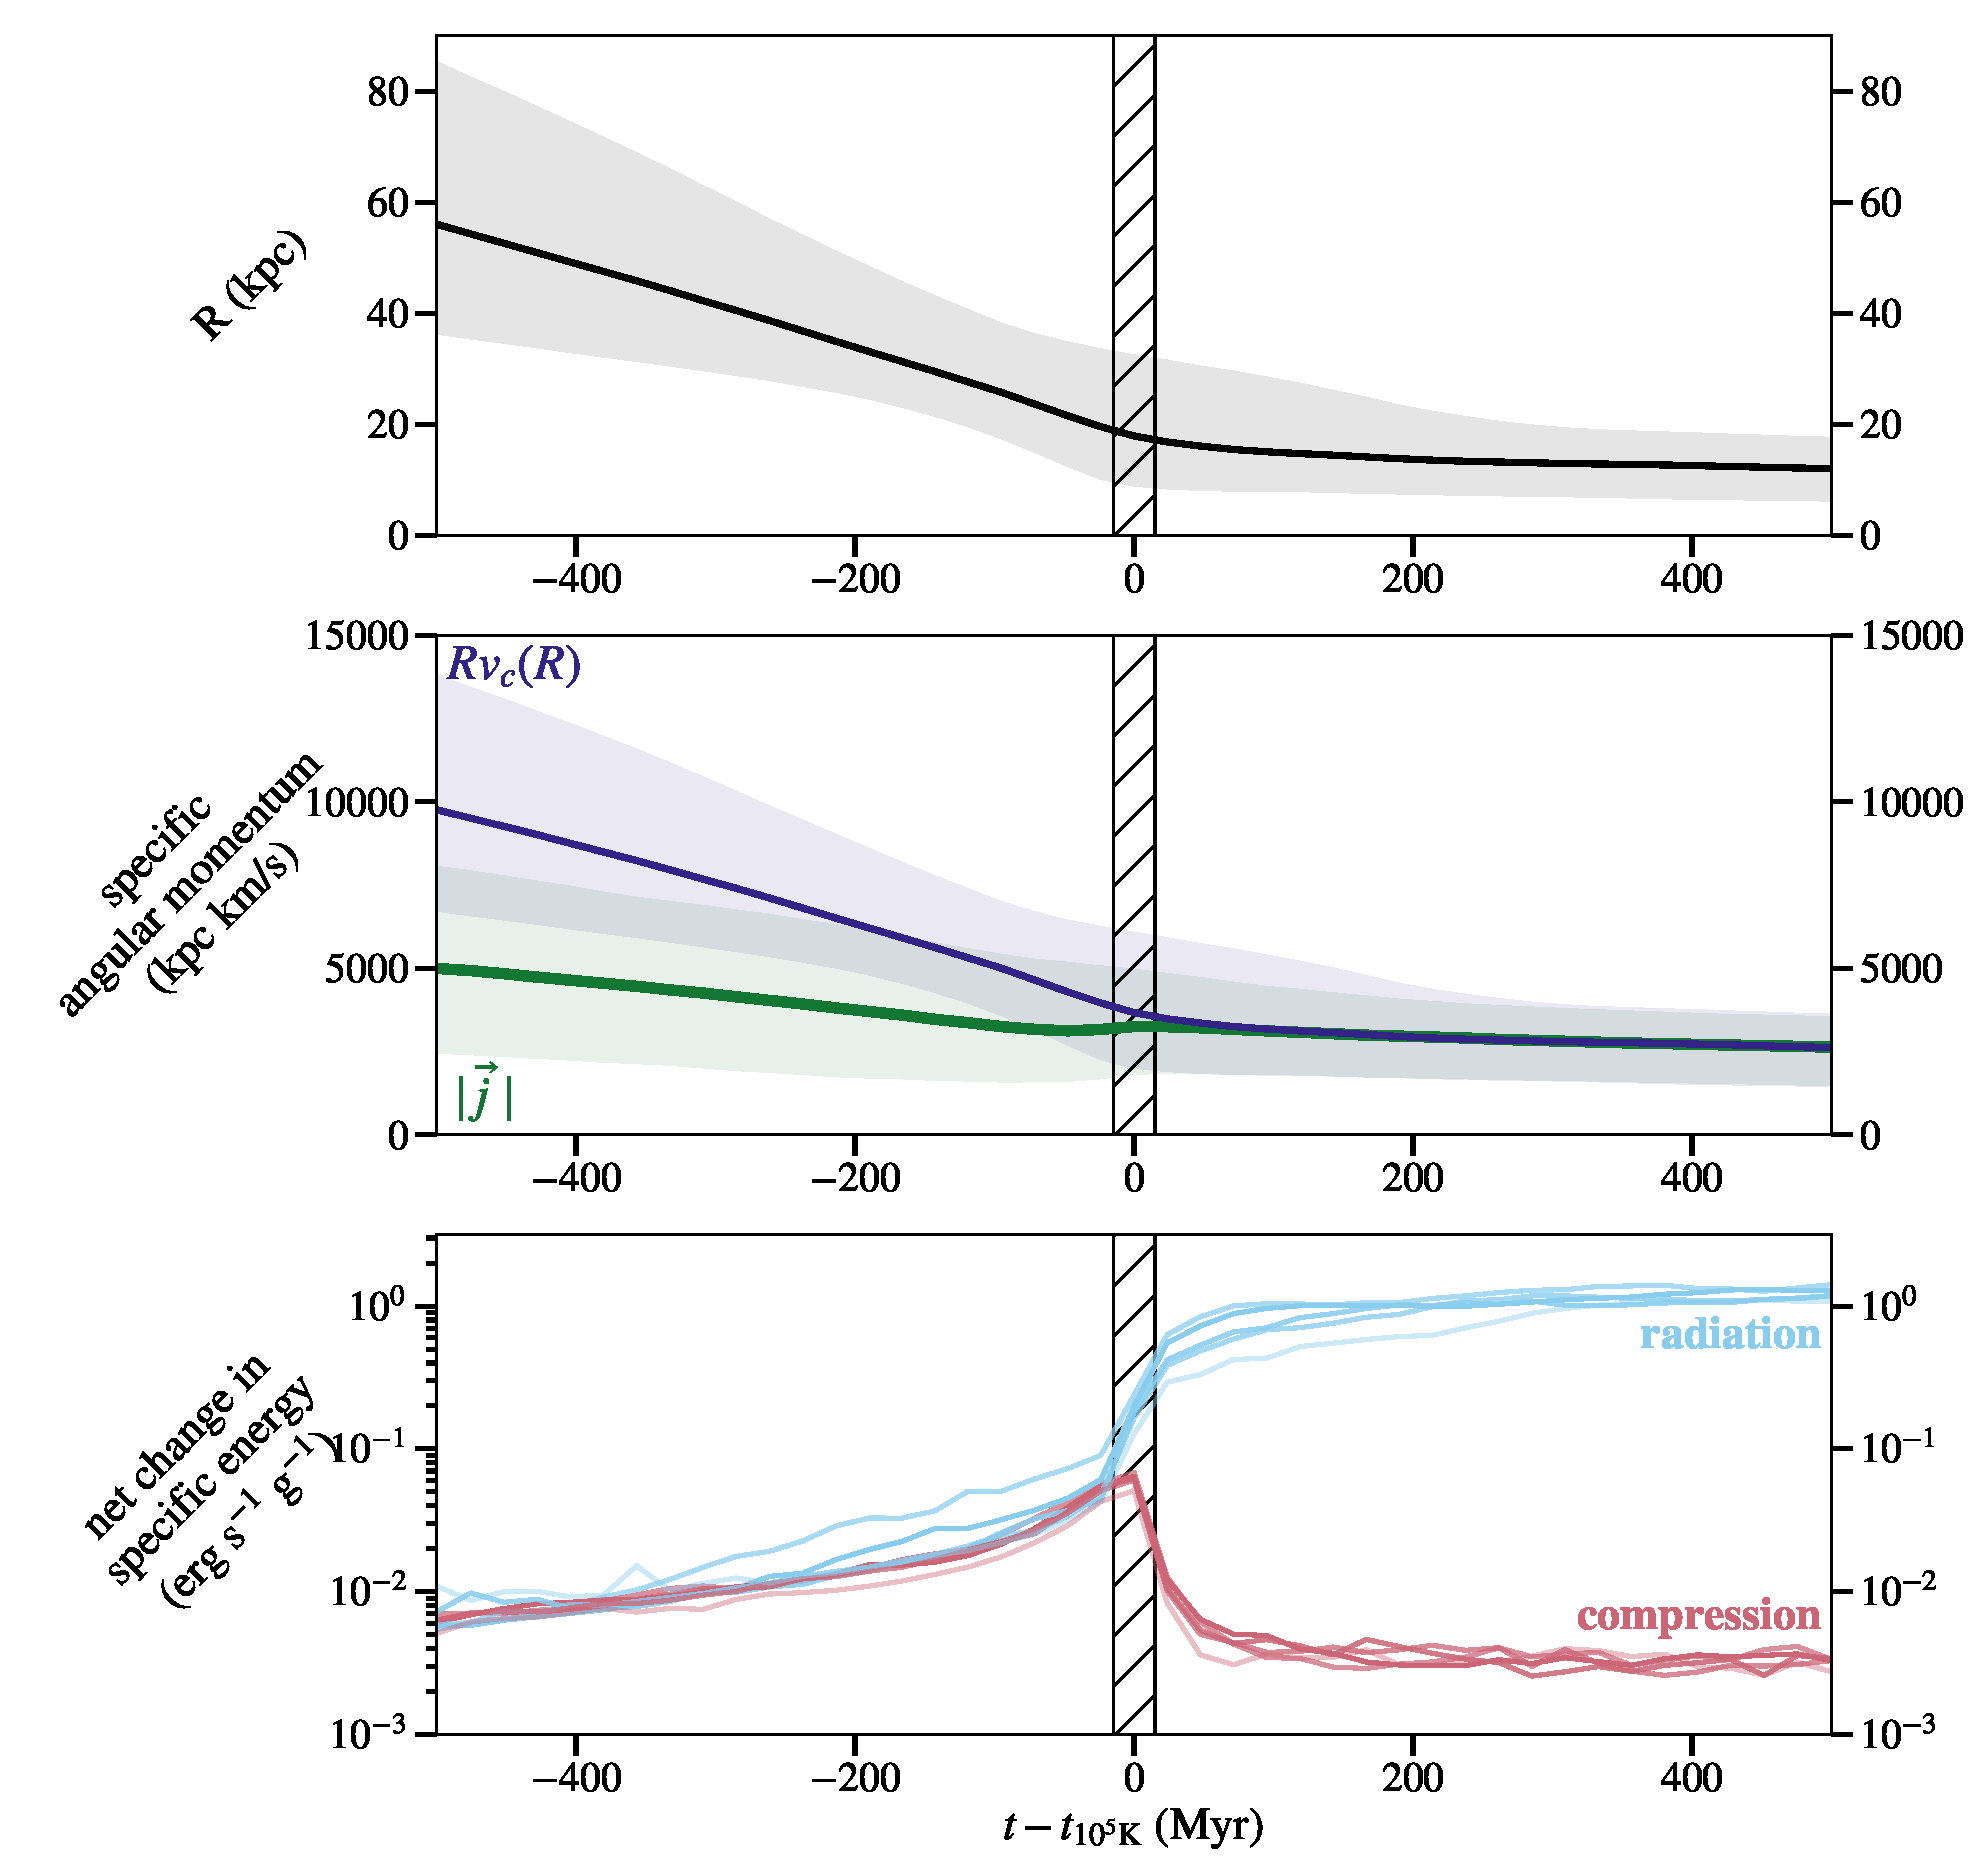
\includegraphics[width=\textwidth]{figures/rad_vs_compress.pdf}
\caption{
\textbf{Top:}
Radius versus time for 1 Gyr centered the time each individual particle cools ($t_{\rm 10^5 K}$).
Solid line is the median radius and shaded region shows the 16th to 84th interval among particles.
Gas moves inward smoothly until it cools, afterwards it moves inward much more slowly.
\textbf{Middle:}
Same as top but for the specific angular momentum of particles (green) and the the value of angular momentum needed to provide full rotational support ($Rv_c(R)$, purple).
Gas becomes fully rotationally-supported at the time it cools, contributing to the slower inward movement shown in the top panel.
\textbf{Bottom:}
Energy loss from radiative cooling (blue) and heating from $PdV$ work on the gas particles (red).
Each line represents the total change in specific energy for particles that cool at the same time (i.e. the same 250 Myr bin in $t_{\rm 10^5 K}$).
Prior to being rotationally-supported the gas cooling is offset by compressive heating, but lack of inward movement decreases the compressive heating afterwards while radiative cooling increases greatly due to increased density.
\textbf{
Make sure cutting out of low-n bins is justified.
Check bin width.
Add comment about the degeneracy/complementarity(?) of increased density and running into the pre-existing gas.
A confusing part to some (e.g. Alex) is how the pole-gas interacts with the rest of the gas.
Whether or not virialization matters depends on when alignment happens. If out in the halo then the virialized halo can circularize. Otherwise it's just gas that circularizes at a given radius when it starts to interact with other gas.
}
}
\label{f:before_after_cooling}
\end{figure*}

\begin{figure}
\centering
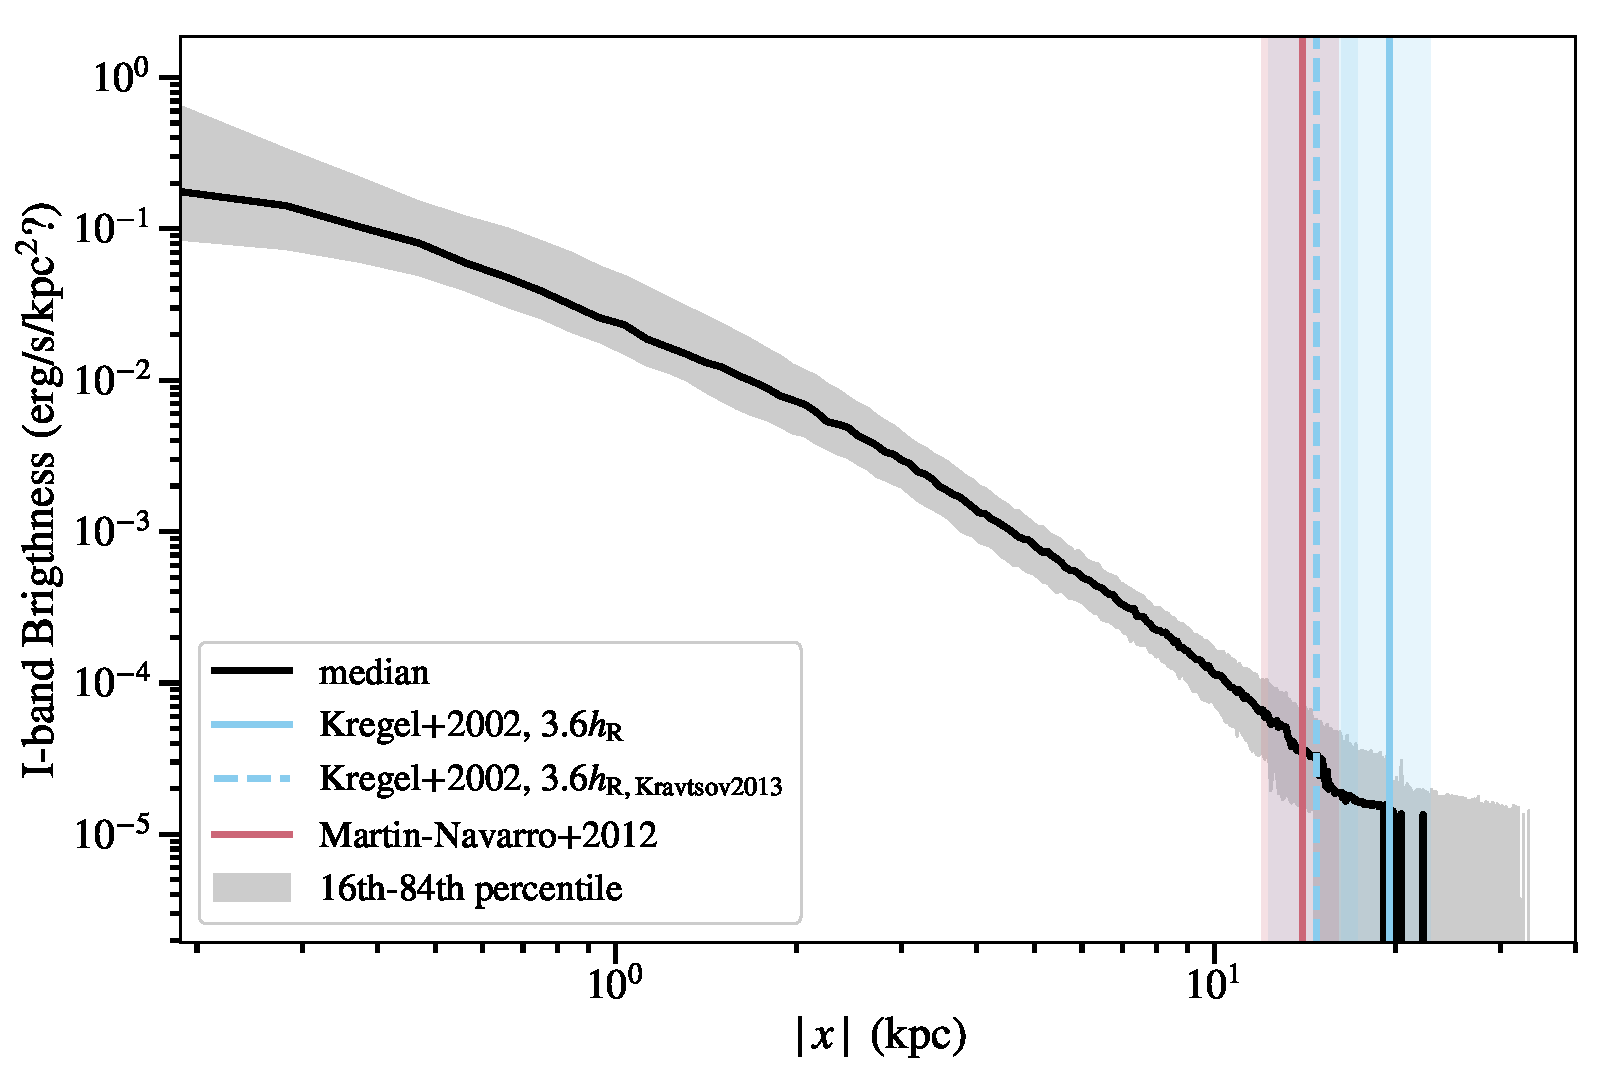
\includegraphics[width=\columnwidth]{figures/brightness_profile.pdf}
\caption{
I-band surface brightness profile for an edge-on stellar disk.
Black line (shaded region) is the median (16th-84th percentile) brightness among pixels 7.5 kpc above/below the disk.
The disk truncates at $\approx 12$ kpc, as seen by the sharp drop-off in the brightness for the percentiles, consistent with observations.
\textbf{
Fill out observations description.
Put on log-linear axis.
Cut out inner radii where dust obscuration is likely an issue.
Maybe cut out entirely and just reference Cameron's paper.
Reference Shea and Kareem's papers.
}
}
\label{f:stellar_profile}
\end{figure}

\begin{figure}
    \centering
    % \includegraphics{}
    \caption{
    \textbf{Spare figure, but maybe
    cooling emission in X-ray, optical and UV lines vs.\ radius, only from tracked particles
    }
    }
    \label{f:emission}
\end{figure}

% Accretion tracks figure description
\textit{
The main panels of Figure~\ref{f: T vs R} show the paths in temperature-radius and entropy-radius space taken by accreting particles.
}

% Distribution of r1e5
\textit{
As an explicit example of how far our distribution is from a condensation model, isotropic cooling occurring randomly within $R_{\rm vir}$ would cool in a wide distribution with a median at $0.8 R_{\rm vir}$, while for our accreted gas the median $\Rcon \approx 0.06 R_{\rm vir}$.
}
\textit{We added all particles with $\Rcon>100$ to $R=100$ bin, so we don't ignore them.}

\subsection{Energetics}

To demonstrate that the hot radial inflow is driven by cooling, we compare the different terms of the energy conservation equation. In steady-state, and assuming the gravitationaly potential is constant,  energy conservation in the radial direction dictates \citep[e.g.][]{Shu82}
\begin{equation}\label{e:energy}
    \rho g v_r + H_{\rm feedback} - \frac{d}{dr}(v_r P)= 
    \frac{d}{dr}\left(\rho v_r \left(\epsilon+\frac{1}{2}v^2\right)\right)  +  \nH^2\Lambda  
\end{equation}
where the terms on the left hand side are the `source terms' -- gravity, feedback, and the work done on the shell by adjacent shells, while the terms on the right represent respectively the heating and acceleration of the flow and radiative losses. 
Integrating over radial shells and rearranging we get the energy integral
\begin{equation}
    \Mdot\frac{d}{dr}\left(\Phi+\frac{3}{2}\epsilon + \frac{1}{2}v^2\right) = 4\pi r^2 \left(\langle\nH^2\Lambda\rangle-\langle H_{\rm feedback}\rangle\right)
\end{equation}

In Fig.~\ref{f:Edot} we plot each of the terms in eqn.~(\ref{e:energy}), averaged over radial shells and over time. Shell averages of quantity $Q$ are calculated via 
\begin{equation}
    \frac{d\dot{E}_Q}{d r} = \frac{\int_{\rm shell} Q\rho^{-1} dm}{\Delta r} 
\end{equation}
where the intergral is over all particles within the shell and $\Delta r$ is the thickness of the shell. The factor $\rho^{-1}$ is since eqn.~\ref{e:energy} is in Eulerian form. We then take the average of all shells at a given $r$ in snapshots of the last Gyr of the simulation. 
% In order to calculate the compression term from a single snapshot, we make the following further approximation \textbf{(TBD: check if justified)}
% \begin{equation}
%     \frac{d\dot{E}_{\rm comp}}{d r} \approx 
%     \Mdot P \left\langle\frac{d V}{d r}\right\rangle_{\rho v_r} \approx
%     \Mdot P \frac{d\langle V \rangle_{\rho v_r} }{dr}
% \end{equation}
% Note that since $d\ln\rho/ d\ln r$ is of order unity, and in hot virial temperature gas $\epsilon/r \approx c_{\rm s}^2/r \approx v_{\rm c}^2/r = g$, we get that $\dot{E}_{\rm comp}$ (eqn.~\ref{e:Ecomp}) and $\dot{E}_{\rm grav}$ (eqn.~\ref{e:Egrav}) are of the same order.
\section{Discussion}

\textbf{
Check the following picture, suggested by James:
Far enough out in an m11 the inner halo is virialized, and compressive heating can contribute comparably to cooling.
This would suggest the cooling radius is max( edge of the virialized area, angular momentum radius), potentially true across all halo masses MW and below.
Can be checked by making an equivalent to Figure~\ref{f:before_after_cooling} for an m11.
}

\textbf{
Consider making slice movies of the galaxy and inner halo to better track how the hot halo affects accretion.
}

\subsection{Generality of accretion mode}

\subsection{Contrast with other accretion mechanisms}

\subsubsection{Condensation/Precipitation}

\begin{itemize}
    \item Nelson+20
    \item Esmerian+20
\end{itemize}
emphasize cold clouds due to over-densities heat back up and join the hot inflow, as in Illustris (see fig.~12 in Nelson+20

\subsubsection{filaments}
Kretschmer+20

\textbf{Discuss resolution effects and Balbus\&Soker}

\subsection{AGN feedback}

\textit{
\begin{itemize}
    \item Results expected to be valid after disc forms (Paper III) and before AGN feedback kicks in (ref.~Byrne+)
    \item Results are baseline for detecting effects of feedback in observations / simulations
\end{itemize}
}

\subsection{Contrast with Cameron+2021}

\textbf{
Discussion goal:
A brief description of gas accretion in FIRE for both CR and non-CR halos, i.e. we have the narrative laid out consistently.
There are two areas where I think the narrative could use some sharpening.
Other goals?
}

% CR vs MHDCV
\textbf{Gas should be moving inward more slowly due to extra support, and so should be a bit cooler ($T\sim 10^5$ K), but otherwise same general picture.}

% Organization into disk: angular momentum exchange
\textbf{
Our analysis suggests that as part of a hot halo with gas moving at sub-sonic speeds angular momentum can be exchanged between gas at all angles.
Therefore, when the gas eventually cools it naturally organizes into a disk.
}
\textbf{
Similar for CR, but gas starts to organize into a disk earlier
}

%  Organization into disk: cooling mechanism
\textbf{Option 1: Radiative cooling is no longer offset by compression.}
\textbf{Option 2: Pile-up increases density, and runaway cooling happens.}

% Does this set the size for disks?

% Results overlap
\textbf{Cameron Fig 7/Fig 3.}
\textbf{Cameron Fig 5/Fig 4.}
\textbf{Cameron Fig 8/Fig 2.}
I think these potential overlaps are fine, and if anything beneficial to reinforce.

\section{Conclusions}

\textbf{TBD.}

\section*{Acknowledgements}

\textbf{TBD.}


%%%%%%%%%%%%%%%%%%%%%%%%%%%%%%%%%%%%%%%%%%%%%%%%%%

%%%%%%%%%%%%%%%%%%%% REFERENCES %%%%%%%%%%%%%%%%%%

% The best way to enter references is to use BibTeX:

\bibliographystyle{mnras}
\bibliography{example} % if your bibtex file is called example.bib

% Alternatively you could enter them by hand, like this:
% This method is tedious and prone to error if you have lots of references
%\begin{thebibliography}{99}
%\bibitem[\protect\citeauthoryear{Author}{2012}]{Author2012}
%Author A.~N., 2013, Journal of Improbable Astronomy, 1, 1
%\bibitem[\protect\citeauthoryear{Others}{2013}]{Others2013}
%Others S., 2012, Journal of Interesting Stuff, 17, 198
%\end{thebibliography}

%%%%%%%%%%%%%%%%%%%%%%%%%%%%%%%%%%%%%%%%%%%%%%%%%%

%%%%%%%%%%%%%%%%% APPENDICES %%%%%%%%%%%%%%%%%%%%%

\appendix

\section{Dependence on Deposited Mass}

\begin{figure}
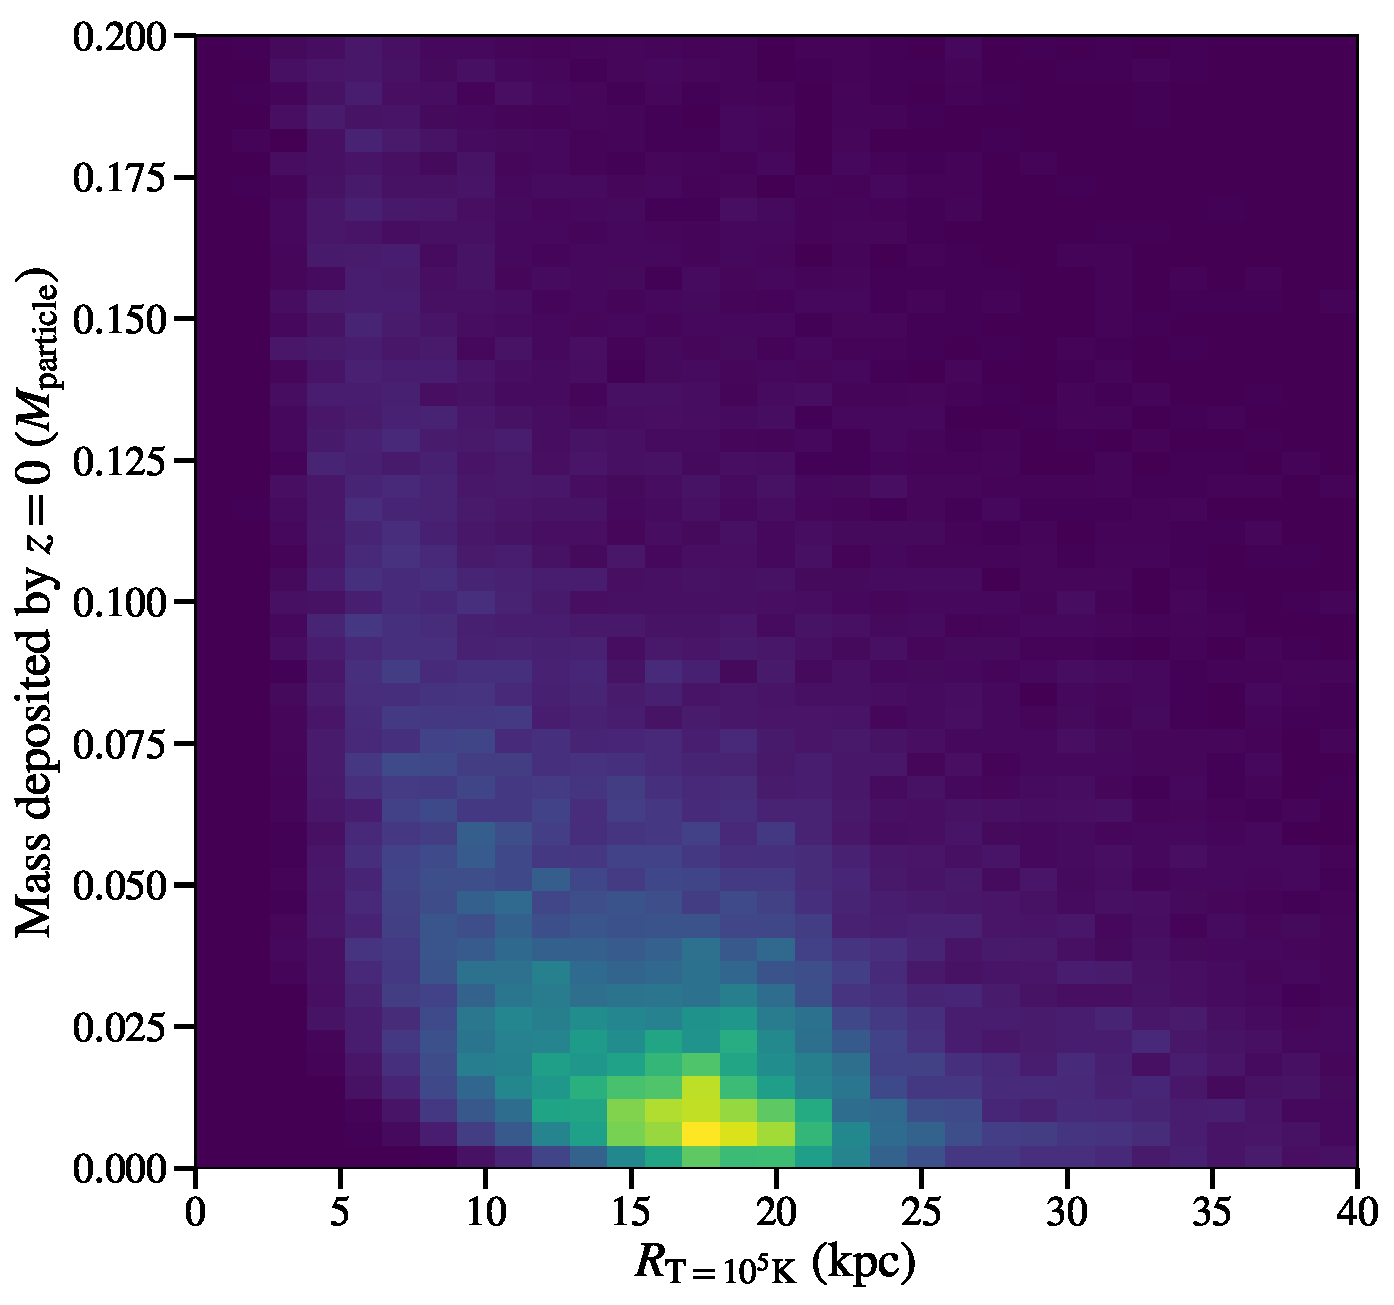
\includegraphics[width=\columnwidth]{figures/mass_dep_vs_R1e5.pdf}
\label{f: deposited mass vs R1e5}
\end{figure}

\section{Angular Momentum of Accreting Material}

% \begin{figure}
%     \centering
%     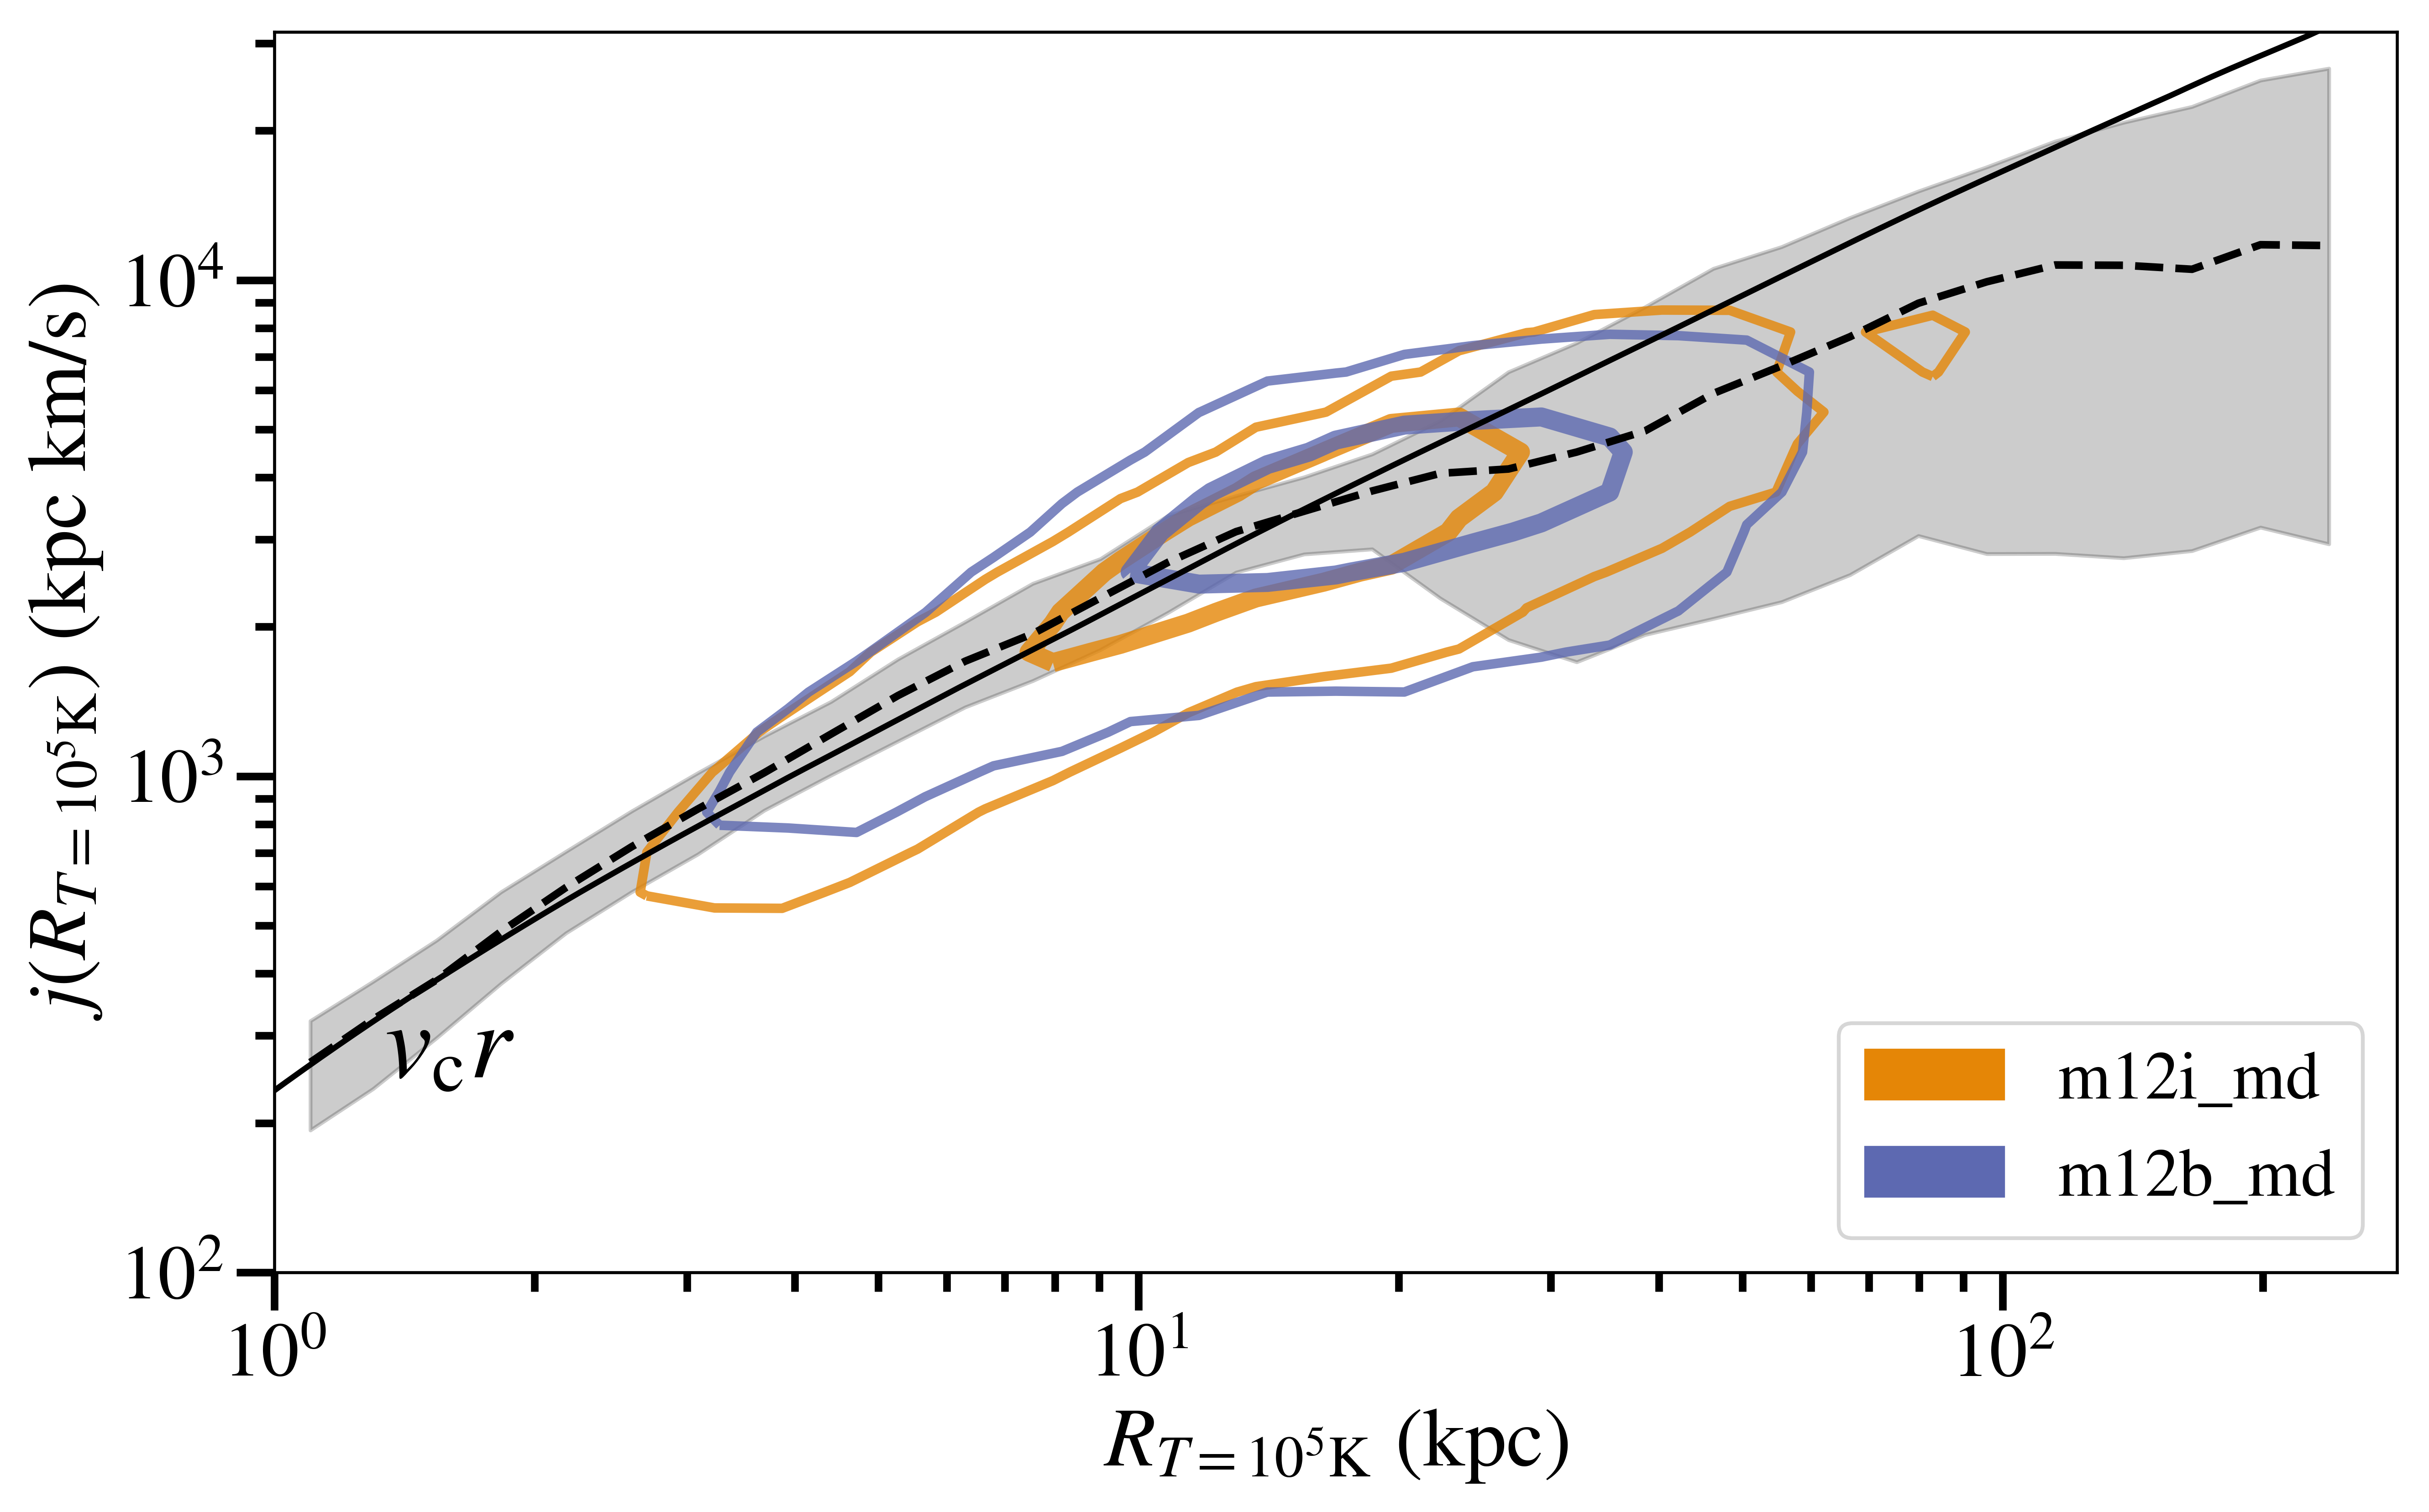
\includegraphics[width=\columnwidth]{figures/j_vs_rcondense.png}
%     \caption{
%     Distribution of $\Rcon$ vs j($\Rcon$) for four FIRE-2 halos with $L(z=0) \sim L^\star$.
% Thick (thin) contours enclose values for 50\% (90\%) of the accreted gas particles.
% The angular momentum as a function of radius for all gas in \texttt{m12i} at $z=0$ is displayed as a dashed line (the median) and shaded regions (5th-95th percentiles).
% \textbf{
% Maybe delete this figure later, because it's only relevant for simulations that have a wide distribution of $\Rcon$, which are only the artificially wide non-md runs.
% }
% \textbf{Is the 100 kpc-cooling gas related to satellite galaxies?}
% \textbf{Try changing shaded region to only hot gas instead of all gas.}
% \textbf{Try histogram of r/(j/vc) instead, to demonstrate that that decreases the spread.}
% \textit{
% In all halos the distributions are consistent with $j_{\rm c} = v_{\rm c} r$, i.e. gas cools once circularized.
% This demonstrates that the variable angular momentum of incoming gas drives the width in the $\Rcon$ distribution.
% }
%     }
%     \label{f: jcool vs Rcon}
% \end{figure}

\section{Metal diffusion vs non-metal diffusion vs MHDCV}

\textbf{Plot of distribution $\Rcon$ for m12i and m12i\_md overlapping. Show cooling only happens at large radii in metal diffusion sims.}

\textbf{Add mhdcv comparison.}

%%%%%%%%%%%%%%%%%%%%%%%%%%%%%%%%%%%%%%%%%%%%%%%%%%


% Don't change these lines
\bsp	% typesetting comment
\label{lastpage}
\end{document}

% End of mnras_template.tex
